\section{Diagnosis: the bottleneck is selection}
\label{sec:diagnosis}

\paragraph{Setup.}
All measurements in this paper are re-analyses of one stored scoring pass per
dataset: for every expression we keep every per-proposal quantity the
released scorer computes (semantic scores under four text variants, the GEM
coherence score, mask geometry, pairwise mask IoU, and IoU against ground
truth), so every table, control and ablation below is computed from the same
pass without re-running the encoders. Pools are SAM ViT-H with
$\text{points\_per\_side}=8$ (mean \meanPoolSize{} proposals/image);
features are the released G2L masked-region features; the scorer is the
released HybridGL guidance reimplemented faithfully
(\S\ref{sec:repro}). ``Oracle'' is the pool member with highest IoU against
ground truth.

\paragraph{The pool is not the bottleneck.}
The oracle mask reaches \oracleMIoU\,mIoU on RefCOCO val
(\oracleG/\oracleP\,on RefCOCOg / RefCOCO+), i.e.\ the pool contains a good
mask for \oracleHitPct\,\% of expressions. The released pipeline achieves
\relMIoU. The recoverable mass --- the \emph{oracle gap} --- is thus
\gapMIoU\,mIoU, and the question is what composes it.

\paragraph{Taxonomy of the oracle gap.}
We classify every expression by the relation between the selected and the
oracle mask into correct, under-segmentation, over-segmentation,
wrong-instance (near-disjoint from the referent) and boundary. Table
\ref{tab:taxonomy} shows the result on the four benchmarks. Wrong-instance
selection carries the overwhelming majority of the recoverable IoU
(\wiSharePct\,\% on RefCOCO, \wiShareGPct\,\% on RefCOCOg,
\wiSharePPct\,\% on RefCOCO+, and the same ordering on gRefCOCO), while
under-segmentation --- the failure that mask merging and granularity
remedies exist to fix --- carries \usSharePct\,\%. Wrong-instance failures are
not a near-miss: the selected mask has mean IoU \wrongInstIoU{} against the
referent, while the oracle reaches \oracleWhenWrong. They are
disproportionately spatial references, though modestly so:
\wiSpatialPct\,\% of wrong-instance failures carry a spatial word from the
operator's vocabulary against \spatialWordOverallPct\,\% of all expressions
(\wiParserPct\,\% vs \spatialFracPct\,\% under the stricter relation
grammar the operator actually parses). The decomposition replicates across
released pipelines on the full official splits
(Table~\ref{tab:multipipeline}, \texttt{multipipeline\_diagnosis.json}):
under a threshold definition (wrong-instance = the selected mask is below IoU
$0.5$ while the pool holds a mask at or above it), wrong-instance selection
carries $94.0/94.2/91.8\%$ of the recoverable IoU for the released HybridGL
selection, $95.1/94.2/92.5\%$ for Global-Local, and
$95.4/94.7/93.2\%$ for S+S, all on RefCOCO/RefCOCO+/RefCOCOg. Global-Local reaches $32.95/36.31/41.62$\,mIoU,
within $1.4$ points of its published val rows despite running on the shared
SAM pool rather than its own FreeSOLO pool. MaskCLIP is the contrast: its own
dense-map component pool caps the oracle at $25.2/28.1/31.8$\,mIoU, so its
recoverable gap is pool-limited (wrong-instance share
$24.3/27.3/31.6\%$); the same dense map on the shared SAM pool selects at
$8.2/9.8/11.6$\,mIoU and is again wrong-instance dominated
($96.7/96.3/95.2\%$). S+S~\cite{splus2024}'s released reverse-blur CLIP
selection reaches $29.46/35.35/38.92$\,mIoU with wrong-instance shares
$95.4/94.7/93.2\%$ on the same pool (its published stage-1 pool is
expression-conditioned GroundingDINO+SAM, so its level is cross-harness, but
the gap composition replicates). Its rectangle-prompt option, a second
released visual-prompt configuration, reaches only $8.91/10.20/10.57$\,mIoU
(wrong-instance shares $96.7/96.5/95.3\%$), a measured selection-prompt
sensitivity that preserves the same failure composition.

\paragraph{Two external checks.}
A 2026 zero-shot study~\cite{earlygrounding2026} independently tabulates the
released selectors: its Global-Local ViT-B row is $33.12/35.29/40.08$\,mIoU
against our $32.95/36.31/41.62$, a $0.2$--$1.5$ point agreement on a different
harness. Its MaskCLIP row is $25.62/27.49/30.13$ using SAM proposals, well
above our dense-map component adaptation ($8.21/10.55/14.30$); our row
therefore characterizes the dense-map component pool, not MaskCLIP's
strongest SAM-proposal route. A second check replaces the released selector
with argmax GEM coherence alone, holding the pool and candidates fixed
(\texttt{gem\_selector.json}): it reaches $44.81/32.81/42.20$\,mIoU against
the released $44.82/40.23/50.08$. Coherence alone matches within
$0.01$\,mIoU on RefCOCO but loses $7.4/7.9$ on RefCOCO+/g, so the semantic
term is load-bearing exactly where attribute and compositional language
dominate, consistent with the mid-layer spatial bias measured
by~\cite{blindposition2025}. The diagnosis therefore holds for pipelines
whose pool contains the referent and names the pool as the limit when it does
not. We attacked it with three falsification tests: the MaskCLIP own-pool
result refutes it as a universal claim (pool-limited), the Global-Local
global-local encoder does not repair selection, and the same MaskCLIP selector
on the shared SAM pool is wrong-instance dominated; the claim survives in its
conditional form. The sample-level containment taxonomy above is stricter,
which is why its shares are lower. The distinction matters for what follows: the operator can act
only on the parsed subset, and its gain is exactly there ---
\operatorOnSpatial\,mIoU over the \strataSpatialN{} parsed-spatial
expressions on RefCOCO val, and zero elsewhere by construction --- which is
why the cross-benchmark pattern below is the diagnostic's decisive test.

Two further released same-class pipelines, TAS~\cite{shu2023tas} and
Ref-Diff~\cite{ni2023refdiff}, were subsequently run end-to-end on the full
RefCOCO val split in the released-pipeline reproduction audit: TAS measures
39.50 mIoU / 29.16 oIoU and Ref-Diff 35.77 mean IoU / 36.54 size-weighted
mIoU, both below the shipped row and below the pool-oracle operating point.
These are neutral measurements of the released pipelines, not floors or
criticisms, and they are not pooled with our single-protocol runs. The exact
Global-Local~\cite{yu2023global} FreeSOLO pool remains unavailable: its
weight URL does not resolve and the repository vendors no FreeSOLO code.

\begin{table*}[t]\centering\small
\caption{Oracle-gap decomposition on additional released pipelines, full
official val splits. Each cell is achieved / oracle mIoU; the last column is
the fraction of the recoverable IoU mass carried by wrong-instance selection
(selected IoU $<0.5$ while the pool holds a mask at $\ge0.5$). HybridGL and
Global-Local use the shared SAM ViT-H pool;
Global-Local~\cite{yu2023global} is its released selector on that pool (its own FreeSOLO pool is unavailable);
S+S~\cite{splus2024} is its released reverse-blur and rectangle CLIP
selection options on that pool (its published stage-1 pool is
GroundingDINO+SAM);
MaskCLIP~\cite{zhou2022maskclip} is a dense open-vocabulary segmenter with no
instance pool, so its row uses components of its own value map under a fixed
rule; an independent 2026 table~\cite{earlygrounding2026} reports a
SAM-proposal MaskCLIP at $25.62/27.49/30.13$\,mIoU, so this row is an
adaptation of the dense-map component pool, not that method's strongest
released route, while the same table's Global-Local ViT-B row
($33.12/35.29/40.08$) agrees with ours to within $1.6$\,mIoU. The exact pools are documented
in \S\ref{sec:diagnosis}; TAS and Ref-Diff are run separately in the
released-pipeline reproduction audit and are not pooled here. Per-pipeline
oIoU and its published numbers are recorded in the artifact. All achieved/oracle cells here are
single-protocol (our unified official evaluator); published numbers are
reported separately (Table~\ref{tab:sota}) and labelled as published
(cross-harness), never pooled with these measurements.}
\label{tab:multipipeline}
\begin{tabular}{lccc c}
\toprule
Pipeline & RefCOCO & RefCOCO+ & RefCOCOg & wrong-instance share \\
 & achieved / oracle & achieved / oracle & achieved / oracle & (R / R+ / Rg) \\
\midrule
HybridGL (released) & 44.82 / 82.21 & 40.23 / 82.40 & 50.08 / 79.12 & 94.0/94.2/91.8 \\
Global-Local (SAM) & 32.95 / 82.21 & 36.31 / 82.40 & 41.62 / 79.12 & 95.1/94.2/92.5 \\
MaskCLIP (own pool) & 8.21 / 25.20 & 10.55 / 28.08 & 14.30 / 31.79 & 24.3/27.3/31.6 \\
S+S (SAM) & 29.46 / 82.21 & 35.35 / 82.40 & 38.92 / 79.12 & 95.4/94.7/93.2 \\
S+S (rectangle) & 8.91 / 82.21 & 10.20 / 82.40 & 10.57 / 79.12 & 96.7/96.5/95.3 \\
\bottomrule
\end{tabular}

\end{table*}

\begin{figure}[t]
\centering
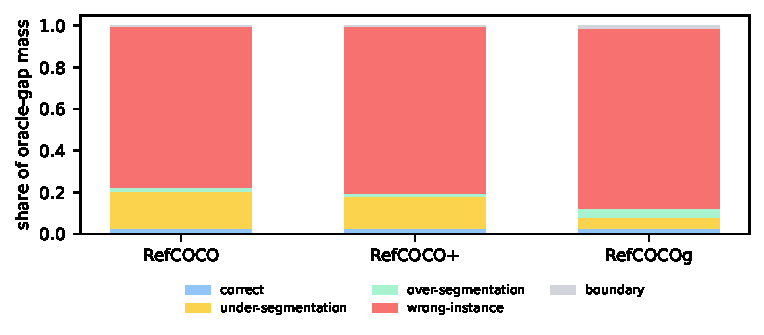
\includegraphics[width=\linewidth]{figures/taxonomy.pdf}
\caption{Share of the oracle-gap mass by error class at the released
operating point, full val splits. Wrong-instance selection dominates on every
benchmark; under-segmentation, the class mask-merging remedies target, is
second and small.}
\label{fig:taxonomy}
\end{figure}

\begin{table}[t]
\centering
\footnotesize
\setlength{\tabcolsep}{4pt}
\caption{Taxonomy of the oracle gap at the released operating point (share of the recoverable IoU in parentheses). Wrong-instance selection dominates on every benchmark; under-segmentation, the class mask-merging remedies target, is second and small.}
\label{tab:taxonomy}
\begin{tabular}{@{}lcccc@{}}
\toprule
split & correct & under-seg. & wrong-inst. & boundary \\
\midrule
RefCOCO (10{,}834) & 0.478\,(0.027) & 0.108\,(0.176) & 0.380\,(0.774) & 0.018\,(0.004) \\
RefCOCO+ (10{,}758) & 0.428\,(0.028) & 0.106\,(0.152) & 0.437\,(0.801) & 0.015\,(0.004) \\
RefCOCOg (4{,}896) & 0.552\,(0.028) & 0.029\,(0.052) & 0.356\,(0.864) & 0.033\,(0.012) \\
\bottomrule
\end{tabular}
\end{table}


\paragraph{Why the released guidance cannot repair them.}
HybridGL's guidance computes relation and coherence terms but ranks only
$\mathrm{topk}(\text{full-expression score}, 3)$; its answer is always one of
those three. On the wrong-instance failures the referent is inside this set
only \oracleInTopThreePct\,\% of the time (mean rank of the oracle:
\meanOracleRank). The same expression scored with its spatial vocabulary
removed --- the \emph{category score} --- puts the referent in its top-8
\goodSetPct\,\% of the time. Candidate-set construction, not the guidance
machinery, is the binding constraint; a perfect chooser restricted to the
released top-3 still reaches \topThreeCeiling\,mIoU, \topThreeCeilingRatio$\times$
the gain the released pipeline actually realizes over argmax
(\relMIoU\,vs \argmaxMIoU) --- almost all of the released gain is the one
structural widening of the candidate set that its top-3 confinement allows.

\paragraph{Where proposal quality \emph{does} matter.}
The residual gap not explained by selection is granularity:
\usSharePct\,\% of the recoverable IoU sits in masks of the correct instance
that stop short of the referent, plus a small boundary class. This is the
second error class our second repair targets.

\paragraph{Pool density does not explain the diagnosis.}
Re-running the released pipeline with SAM at $\text{points\_per\_side}=16$ on
a fixed \ppsN-expression sample (\ppsProposalDelta\,\% more proposals) raises
the oracle by only \ppsOracleDelta\,mIoU while the released pipeline loses
\ppsGuidedDelta\,mIoU --- a denser pool adds distractors and concentrates
selection failure rather than repairing it. The wrong-instance share of the
gap is stable (\ppsWiEight\,$\to$\,\ppsWiSixteen) and the operator's gain is
stable too (\ppsOursEight\,$\to$\,\ppsOursSixteen). Evidence:
\texttt{pool\_robustness.json}.
